\section{moeo\-Combined\-MOLS$<$ EOT $>$ Class Template Reference}
\label{classmoeoCombinedMOLS}\index{moeoCombinedMOLS@{moeoCombinedMOLS}}
This class allows to embed a set of local searches that are sequentially applied, and so working and updating the same archive of non-dominated solutions.  


{\tt \#include $<$moeo\-Combined\-MOLS.h$>$}

Inheritance diagram for moeo\-Combined\-MOLS$<$ EOT $>$::\begin{figure}[H]
\begin{center}
\leavevmode
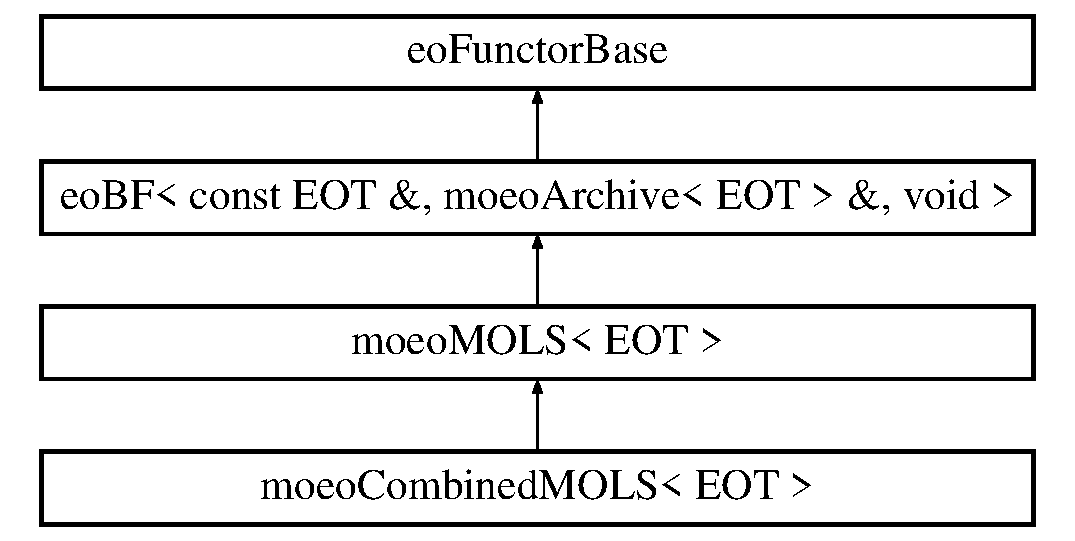
\includegraphics[height=4cm]{classmoeoCombinedMOLS}
\end{center}
\end{figure}
\subsection*{Public Member Functions}
\begin{CompactItemize}
\item 
{\bf moeo\-Combined\-MOLS} ({\bf eo\-Eval\-Func}$<$ EOT $>$ \&\_\-eval, {\bf moeo\-MOLS}$<$ EOT $>$ \&\_\-first\_\-ls)
\begin{CompactList}\small\item\em Ctor. \item\end{CompactList}\item 
void {\bf add} ({\bf moeo\-MOLS}$<$ EOT $>$ \&\_\-ls)
\begin{CompactList}\small\item\em Adds a new local search to combine. \item\end{CompactList}\item 
void {\bf operator()} (const EOT \&\_\-eo, {\bf moeo\-Archive}$<$ EOT $>$ \&\_\-arch)
\begin{CompactList}\small\item\em Gives a new solution in order to explore the neigborhood. \item\end{CompactList}\end{CompactItemize}
\subsection*{Private Attributes}
\begin{CompactItemize}
\item 
{\bf eo\-Eval\-Func}$<$ EOT $>$ \& {\bf eval}\label{classmoeoCombinedMOLS_b2c0866a1808022bd3a9dac89e528a01}

\begin{CompactList}\small\item\em the full evaluator of a solution \item\end{CompactList}\item 
std::vector$<$ {\bf moeo\-MOLS}$<$ EOT $>$ $\ast$ $>$ {\bf combined\-MOLS}\label{classmoeoCombinedMOLS_a5ccc182c0d61421fc524c2da3671099}

\begin{CompactList}\small\item\em the vector that contains the combined MOLS \item\end{CompactList}\end{CompactItemize}


\subsection{Detailed Description}
\subsubsection*{template$<$class EOT$>$ class moeo\-Combined\-MOLS$<$ EOT $>$}

This class allows to embed a set of local searches that are sequentially applied, and so working and updating the same archive of non-dominated solutions. 



Definition at line 24 of file moeo\-Combined\-MOLS.h.

\subsection{Constructor \& Destructor Documentation}
\index{moeoCombinedMOLS@{moeo\-Combined\-MOLS}!moeoCombinedMOLS@{moeoCombinedMOLS}}
\index{moeoCombinedMOLS@{moeoCombinedMOLS}!moeoCombinedMOLS@{moeo\-Combined\-MOLS}}
\subsubsection{\setlength{\rightskip}{0pt plus 5cm}template$<$class EOT$>$ {\bf moeo\-Combined\-MOLS}$<$ EOT $>$::{\bf moeo\-Combined\-MOLS} ({\bf eo\-Eval\-Func}$<$ EOT $>$ \& {\em \_\-eval}, {\bf moeo\-MOLS}$<$ EOT $>$ \& {\em \_\-first\_\-ls})\hspace{0.3cm}{\tt  [inline]}}\label{classmoeoCombinedMOLS_9305380cd8f5a4d85ef603fa85c1860b}


Ctor. 

\begin{Desc}
\item[Parameters:]
\begin{description}
\item[{\em \_\-eval}]the full evaluator of a solution \item[{\em \_\-first\_\-ls}]the first multi-objective local search to add \end{description}
\end{Desc}


Definition at line 33 of file moeo\-Combined\-MOLS.h.

References moeo\-Combined\-MOLS$<$ EOT $>$::combined\-MOLS.

\subsection{Member Function Documentation}
\index{moeoCombinedMOLS@{moeo\-Combined\-MOLS}!add@{add}}
\index{add@{add}!moeoCombinedMOLS@{moeo\-Combined\-MOLS}}
\subsubsection{\setlength{\rightskip}{0pt plus 5cm}template$<$class EOT$>$ void {\bf moeo\-Combined\-MOLS}$<$ EOT $>$::add ({\bf moeo\-MOLS}$<$ EOT $>$ \& {\em \_\-ls})\hspace{0.3cm}{\tt  [inline]}}\label{classmoeoCombinedMOLS_bd6b8f46211d5d531753c69fcd76cba4}


Adds a new local search to combine. 

\begin{Desc}
\item[Parameters:]
\begin{description}
\item[{\em \_\-ls}]the multi-objective local search to add \end{description}
\end{Desc}


Definition at line 43 of file moeo\-Combined\-MOLS.h.

References moeo\-Combined\-MOLS$<$ EOT $>$::combined\-MOLS.\index{moeoCombinedMOLS@{moeo\-Combined\-MOLS}!operator()@{operator()}}
\index{operator()@{operator()}!moeoCombinedMOLS@{moeo\-Combined\-MOLS}}
\subsubsection{\setlength{\rightskip}{0pt plus 5cm}template$<$class EOT$>$ void {\bf moeo\-Combined\-MOLS}$<$ EOT $>$::operator() (const EOT \& {\em \_\-eo}, {\bf moeo\-Archive}$<$ EOT $>$ \& {\em \_\-arch})\hspace{0.3cm}{\tt  [inline, virtual]}}\label{classmoeoCombinedMOLS_fa7de12db00b89feb139372603bba4aa}


Gives a new solution in order to explore the neigborhood. 

The new non-dominated solutions are added to the archive \begin{Desc}
\item[Parameters:]
\begin{description}
\item[{\em \_\-eo}]the solution \item[{\em \_\-arch}]the archive of non-dominated solutions \end{description}
\end{Desc}


Implements {\bf eo\-BF$<$ const EOT \&, moeo\-Archive$<$ EOT $>$ \&, void $>$}.

Definition at line 54 of file moeo\-Combined\-MOLS.h.

References moeo\-Combined\-MOLS$<$ EOT $>$::combined\-MOLS, and moeo\-Combined\-MOLS$<$ EOT $>$::eval.

The documentation for this class was generated from the following file:\begin{CompactItemize}
\item 
moeo\-Combined\-MOLS.h\end{CompactItemize}
